\setcounter{step}{0}
%------------------------------------------
% information doc
\subsection{Pizza}
%------------------------------------------

\begin{ingredient}
%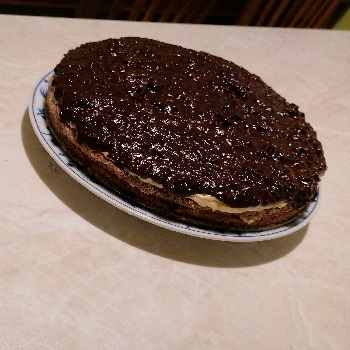
\includegraphics[height=5.5cm]{images/daim}
\def\portions{4}%
\textbf{{\normalsize Ingrediencie (\portions porcie):}}
%\vspace{0.5cm}
\begin{main}
	\item šunka
	\item syr
	\item paradajkový pretlak
	\item pizza korenie, oregáno
	\item cibuľa
	\item vajíčko (potom ale pečieme pomalšie)
\end{main}
\begin{subingredient}{Cesto}
	\item 1 cà.c de test1
	\item 1 à 2 cà.S de test2
	\item 3 gouttes de test3
	\item 8 morceaux de test4.	
\end{subingredient}

\begin{subingredient}{Syrová omáčka}
	\item niva/rival
	\item syr v črievku
	\item smotana na varenie/na šľahanie
	\item nastrúhaný syr
\end{subingredient}
\end{ingredient}
\begin{recipe}
\textbf{{\normalsize Príprava:}}
\begin{enumerate}

\item{Urobíme cesto:}
\begin{enumerate}
\item{Blabla}
\item{Blabla}
\item{Blabla}
\item{Blabla}
\end{enumerate}
\item{Na cesto dáme veci, podľa chuti}

\item{Syrová pizza:}
\begin{enumerate}
\item{Postrúhame tvrdý syr}
\item{zmiešame so smotanou, plesnivým syrom, syrom v črievku}
\item{Natrieme na pizzu}
\end{enumerate}

\end{enumerate}
\end{recipe}

\begin{notes}

\end{notes}
\clearpage	